\chapter{Diseños individuales para la iteración competitiva de Alberto Alejandro Rivas Fernandez}
\label{ape:disenyoAlberto}

En este apéndice se muestran los diseños individuales realizados por Alberto Alejandro Rivas Fernandez para la iteración competitiva.

\begin{figure}[ht!]
  \centering
  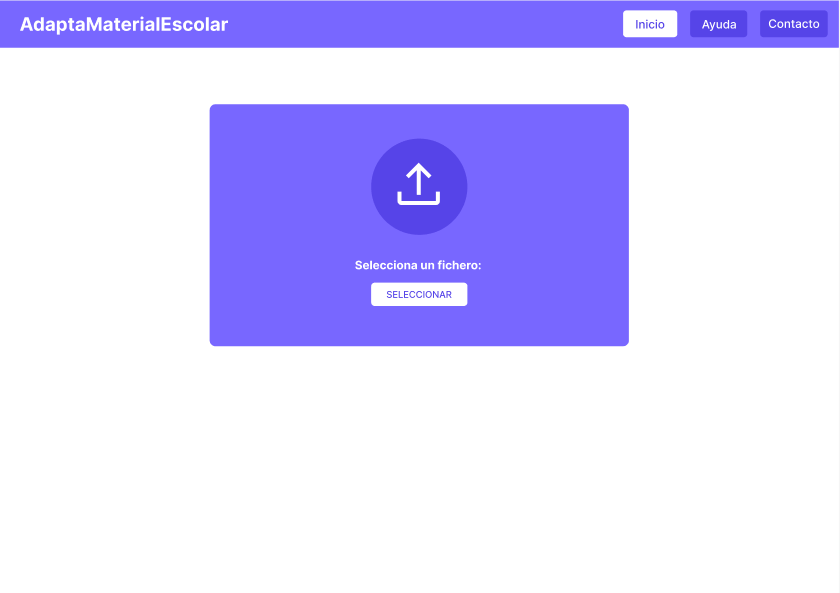
\includegraphics[width=0.6\textwidth]{Diseño/Alberto/PaginaPrincipal1.PNG}
  \caption{Diseño página principal de Alberto.}
  \label{AlbertoPaginaPrincipal1}
\end{figure}

\begin{figure}[ht!]
  \centering
  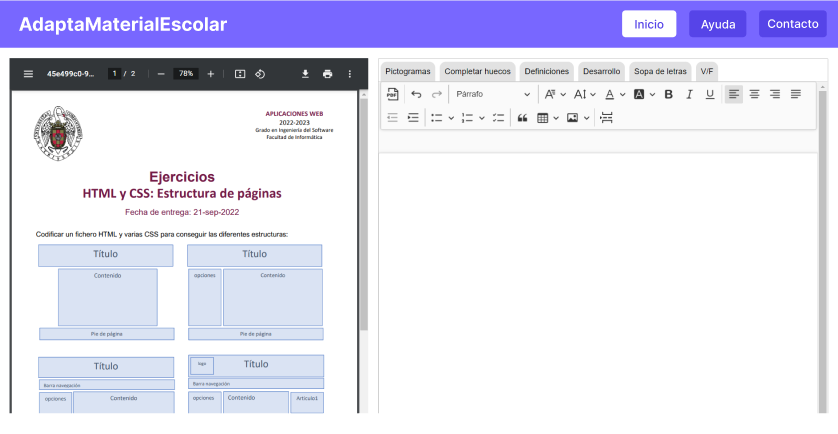
\includegraphics[width=0.6\textwidth]{Diseño/Alberto/PaginaPrincipal2.PNG}
  \caption{Diseño página principal de Alberto.}
  \label{AlbertoPaginaPrincipal2}
\end{figure}


\begin{figure}[ht!]
  \centering
  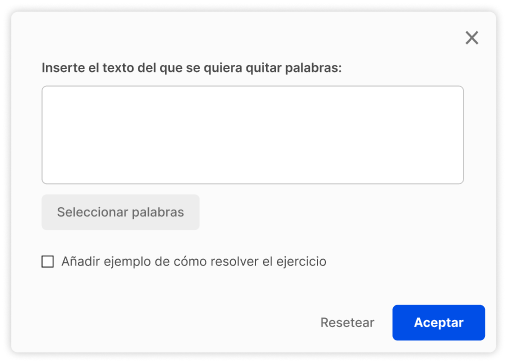
\includegraphics[width=0.6\textwidth]{Diseño/Alberto/Capture13.PNG}
  \caption{Diseño de ejercicios con huecos de Alberto.}
  \label{Alberto13}
\end{figure}

\begin{figure}[ht!]
  \centering
  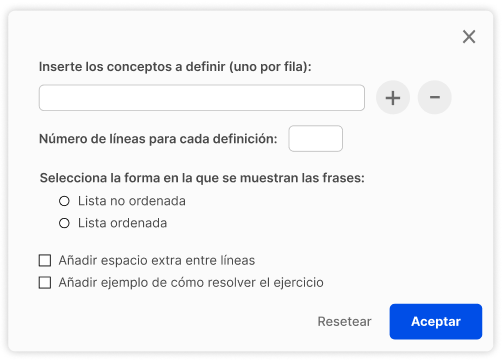
\includegraphics[width=0.6\textwidth]{Diseño/Alberto/Capture14.PNG}
  \caption{Diseño de ejercicios de definiciones de Alberto.}
  \label{Alberto14}
\end{figure}

\begin{figure}[ht!]
  \centering
  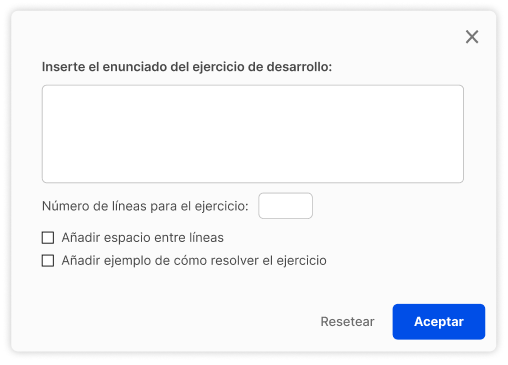
\includegraphics[width=0.6\textwidth]{Diseño/Alberto/Capture15.PNG}
  \caption{Diseño de ejercicios de desarrollo de Alberto.}
  \label{Alberto15}
\end{figure}

\begin{figure}[ht!]
  \centering
  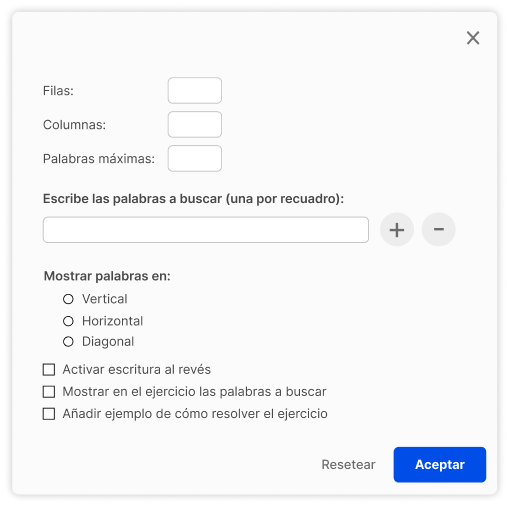
\includegraphics[width=0.6\textwidth]{Diseño/Alberto/Capture16.PNG}
  \caption{Diseño de ejercicios de sopa de letras de Alberto.}
  \label{Alberto16}
\end{figure}

\begin{figure}[ht!]
  \centering
  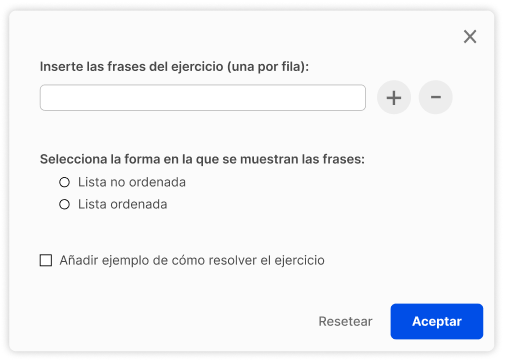
\includegraphics[width=0.6\textwidth]{Diseño/Alberto/Capture17.PNG}
  \caption{Diseño de ejercicios de verdadero y falso de Alberto.}
  \label{Alberto17}
\end{figure}


\begin{figure}[ht!]
  \centering
  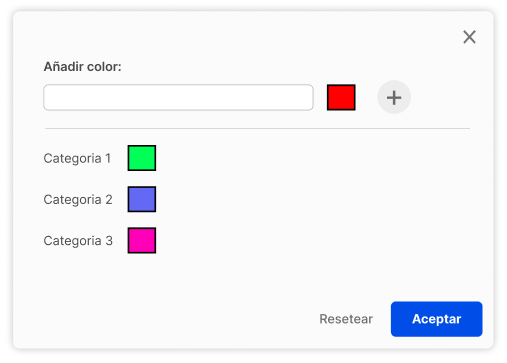
\includegraphics[width=0.6\textwidth]{Diseño/Alberto/Capture01.PNG}
  \caption{Diseño de leyenda de colores de Alberto.}
  \label{Alberto1}
\end{figure}

\begin{figure}[ht!]
  \centering
  
\includegraphics[width=0.6\textwidth]{Diseño/Alberto/Capture02.PNG}
  \caption{Diseño de leyenda de colores por asignatura de Alberto.}
  \label{Alberto2}
\end{figure}

\begin{figure}[ht!]
  \centering
  
\includegraphics[width=0.6\textwidth]{Diseño/Alberto/Capture03.PNG}
  \caption{Diseño de cuatrícula de Alberto.}
  \label{Alberto3}
\end{figure}

\begin{figure}[ht!]
  \centering
  
\includegraphics[width=0.6\textwidth]{Diseño/Alberto/Capture04.PNG}
  \caption{Diseño de doble pauta de Alberto.}
  \label{Alberto4}
\end{figure}

\begin{figure}[ht!]
  \centering
  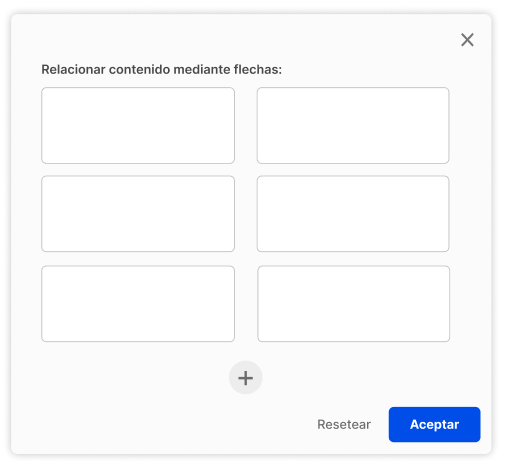
\includegraphics[width=0.6\textwidth]{Diseño/Alberto/Capture05.PNG}
  \caption{Diseño de ejercicio de flechas de Alberto.}
  \label{Alberto5}
\end{figure}

\begin{figure}[ht!]
  \centering
  
\includegraphics[width=0.6\textwidth]{Diseño/Alberto/Capture06.PNG}
  \caption{Diseño de ejercicios de matemáticas con huecos de Alberto.}
  \label{Alberto6}
\end{figure}

\begin{figure}[ht!]
  \centering
  
\includegraphics[width=0.6\textwidth]{Diseño/Alberto/Capture08.PNG}
  \caption{Diseño de añadir resumen de Alberto.}
  \label{Alberto8}
\end{figure}

\begin{figure}[ht!]
  \centering
  
\includegraphics[width=0.6\textwidth]{Diseño/Alberto/Capture10.PNG}
  \caption{Diseño de pictotraductor de Alberto.}
  \label{Alberto10}
\end{figure}

\begin{figure}[ht!]
  \centering
  
\includegraphics[width=0.6\textwidth]{Diseño/Alberto/Capture07.PNG}
  \caption{Diseño de ejercicios de espacios para dibujar de Alberto.}
  \label{Alberto7}
\end{figure}

\begin{figure}[ht!]
  \centering
  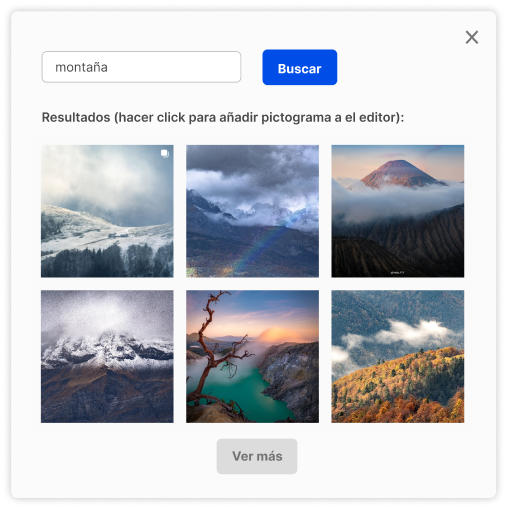
\includegraphics[width=0.6\textwidth]{Diseño/Alberto/Capture12.PNG}
  \caption{Diseño de buscar pictogramas de Alberto.}
  \label{Alberto12}
\end{figure}